\documentclass[12pt,a4paper]{article}
\usepackage[margin=3cm, left=4cm]{geometry}
\usepackage{graphicx}
\usepackage{subfigure}

\title{\textbf{Synopsis}}

\author{Rahul Bali\\16205025\\Department of Computer Science and Engineering\\Punjab Engineering College, Chandigarh}


\date{\today}

\begin{document}
	\maketitle

	\section{Introduction}
	During the last decade, the importance of recommender systems has been increasing to the point that the success of many well-known service providers depends on these technologies. Recommender systems can assist people in their decision making process by anticipating preferences. However, common recommender algorithms often suffer from lack of explicit feedback and the “cold start” problem. This thesis investigates an approach of using implicit data only, to extract users’ intent for fashion e-commerce in cold start situations. Markov Decision Processes (MDPs) are used on web session data to extract topic models. This thesis also explores how well the topic models can capture users intent and whether they can be used to produce good recommendations. The results show that this approach was able to accurately identify sessions topics, and in most cases the topics could successfully be translated to product recommendations.\\

	Recommender systems have become the most popularly unpopular area in the field of machine learning. It is being used widely yet it is behind the noticeable frame of people's vision. Recommender systems have been the major milestones in the application of Computer Science to other areas. This can be categorized into collaborative-filtering, content based RS and some Hybrid Approaches.\\
	
	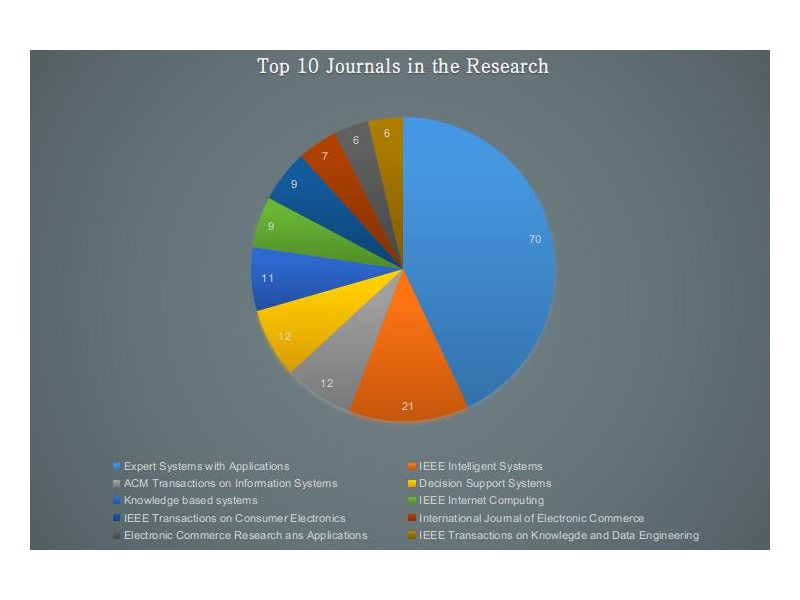
\includegraphics[width=\linewidth]{images/Untitled1.png}\\

Content-based RS focuses on building user profile of a single user for recommendations while collaborative-filtering(CF) RS uses data from fellow users/peers to recommend a particular user. Content-based RS has its roots in Information Retrieval, utility function is defined for each item for a user based on the history of the user purchases, searches, etc. Usually, higher the utility function value, higher is the preference for recommendation. Limited feature Extraction leads to limited possible recommendations. Also, only domain specific recommendations can be inferred. New user problem exists for the both kind of the RS systems. Almost no information is present about the new users into the application environment.\\

Collaborative-filtering techniques create user groups / clusters based on similar tastes / browsing habits, and few techniques consider stereotypes for peer groups. And collaborative-filtering is of two types based on the data mining techniques; heuristics (memory) based, model-based CF. Both techniques have decent application in the industry for real world problem solving. Improvements have been shown in the combined use of these data mining techniques.\\

Improvements over the limitations of the above RS have been implemented using hybrid RS and many extensions of current RS. Current state of the recommender systems can be enhanced by extending the capabilities of RS. One approach highlighted is use of advanced profiling of items and users. Another by the use of Mathematical Approximation Theory and some RBF. Multidimensionality Reduction based on contextual approaches on recommender systems. Multiple rating criterias which help user to rate an item from various perspectives not just one. Making RS less intrusive to a user of the application system, providing some control to the user for change in the
behavior of RS. Improving flexibility of RS, providing language like RQL for handling operations on RS. Measuring how effective RS has been by calculating the results in various fashions.

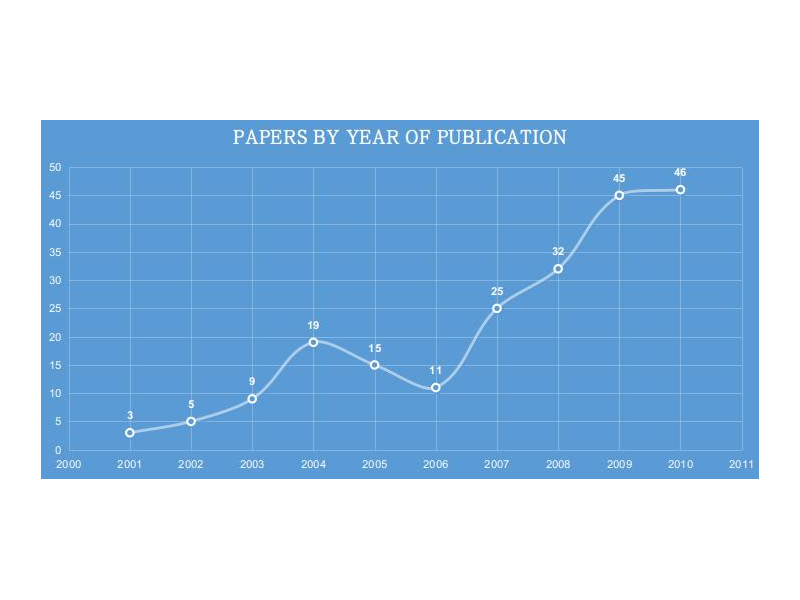
\includegraphics[width=\linewidth]{images/Untitled}\\

In memory-based CF, similarity among users is calculated using cosines of the user matrices. Correlation and similarity are calculated by heuristic techniques.Heuristics basically work by aggregation or summation(∑) of the past activities of the users who are similar to a user for whom recommendations are required. Another is Model-based CF, models are prepared based on ANN, K-means clustering, Gibbs sampling, Probabilistic latent semantic analysis, generative semantics of latent Dirichlet Allocation. CF recommendation systems also faces few issues; new item problem, in which recommendations of this new item are not made to any use because of the shortage of the data. Sparsity, this issue arises for a user whose tastes are fairly diverse from the other users which increases hardness of the recommendations. Demographic-based filtering and preference-based filtering could be helpful with these kind of limitations. Preference-based filtering is currently high on research and industry use.\\

Historically, people have relied on recommendations and mentions
from their peers or the advice of experts to support decisions and discover new material. They discuss the week’s blockbuster over the water cooler, they read reviews in the newspaper’s entertainment section, or they ask a librarian to suggest a book. They may trust their local theater manager or news stand to narrow down their choices, or turn on the TV and watch whatever happens to be playing.
These methods of recommending new things have their limits, particularly for information discovery. There may be an independent film or book that a person would enjoy, but no one in their circle of acquaintances has heard of it yet. There may be a new indie band in another city whose music will likely never cross the local critic’s radar. Computer-based systems provide the opportunity to expand the
set of people from whom users can obtain recommendations. They also
enable us to mine users’ history and stated preferences for patterns that
neither they nor their acquaintances identify, potentially providing a
more finely-tuned selection experience.\\



	\newpage
	\section{Literature Review}
	
	\cite{adomavicius2005toward} talks about the field of recommender system from the generation point of view. It classifies recommender systems into three categories: content-based, collaborative, hybrid recommendation approaches.
	Limitations of the current generation recommender systems and discusses the extensions that are possible recommendations capabilities. Making Recommender systems even broader range of applications. \\
	
	\cite{park2012literature} is reviewing the already existing literature and tries to classify each into recommendation systems research. This paper consists survey of 210 research papers which were selected from 46 Journals. Eight categories of application field and data mining techniques are defined and each paper is then categorized. Application field chosen were books, documents(papers, blogs, web pages), images, movies, music, shopping(online, offline, mobile shopping), TV programs, and others(consists hotel, travel, food). Data mining techniques which were used to classify documents: Association rule mining, clustering, decision tree, k-nearest neighbor, link analysis, neural network, regression, and other heuristic methods. Classification of each paper was done by 2 authors one by one, then other 2 authors made the final verification of the	classified documents.\\
	
	\cite{linden2003amazon} describes the base use of Recommender system technology in the industry sector of the E-commerce applications. Amazon compares their item-to-item collaborative filtering algorithm to the traditional  collaborative filtering, cluster models, and search-based methods. Final algorithm produces recommendations in real-time, scales to massive data sets, and generates high quality recommendations.\\
	
	\cite{sarwar2001item} shows how one can define and implement the Recommender systems for the real world application. Important technique of Matrix Factorization is deployed in theory and in action.\\
	
	\cite{konstan1997grouplens} Grouplens Research undertook the task of achieving non-intrusive technology for getting the explicit ratings. \\
	
	\cite{schein2002methods} Metrics are created to measure the effectiveness of the predictions of the results of recommender systems.\\
	
	\cite{tintarev2011designing} user perspective into the recommendation trust they can have, providing explanation for the way recommendations are provided helps user gain trust into the service.\\
	
	\cite{ricci2011introduction} describes the role of recommender systems for the user and the service providers. Providers have got much inclination to recommender systems which has proved to be beneficial for many past decade.\\
	
	\cite{ekstrand2011collaborative} The differing personalities exhibited by different recommender algorithms show that recommendation is not a one-size-fits-all problem. Specific tasks, information needs, and item domains
	represent unique problems for recommenders, and design and evaluation of recommenders needs to be done based on the user tasks to be supported.\\
	
	
	
	\begin{center}
		\begin{tabular}{ |p{3cm}|p{3cm}|p{0.8cm}|p{4cm}|p{2cm}| }
			\hline
			%\multicolumn{5}{|c|}{Country List} \\
			%\hline
			Author & Source & Year & Findings & Limitation\\
			\hline
			G. Adomavicius, A. Tuzhilin & IEEE Transactions on Knowledge and Data Engineering & 2005 & Various types of recommender systems with their limitations and possible extensions & -\\
			\hline
			D.H. Park et al. & Expert Systems with Applications & 2012 & Only Journals papers used for Survey. Presents the diversity in the RS research. & Research does not include the ME , PhD thesis. No Conference Papers included.\\
			\hline
			G. Linden, B. Smith, J. York & IEEE Internet Computing & 2003 & Amazon's Algorithm performance, Good Scalability & -\\
			\hline
			B. Sarwar et al. & Proceedings of the 10th international conference on World Wide Web & 2001 & Implementation of the Matrix factorization on Recommender Systems & -\\
			\hline
			A. I. Schein et al. & ACM SIGIR conference on Research and development in information retrieval & 2002 & Novel Method of Recommendation and Metric for effectiveness of RS & -\\
			 \hline
			J.A. Konstan et al. & Communications of the ACM & 1997 &  &\\
			 \hline
			N. Tintarev, J. Masthoff & Recommender Systems Handbook & 2011 &  &\\
			 \hline
			M.D. Ekstrand et al. & Foundations and Trends{\textregistered} in Human--Computer Interaction & 2011 &  &\\
			 \hline
			F. Ricci, L. Rokach, B. Shapira & Recommender Systems Handbook & 2011 &  &\\
			\hline
		\end{tabular}
	\end{center}
	
	
	
	\newpage
	\section{Problem Statement}

	Creating new recommender system technology that can quickly produce high quality recommendations, performing many recommendations per second for millions of users and items and achieving high coverage in the face of data sparsity. Meanwhile, tackling the cold start problem in the several different contexts.
	
	\section{Objectives}
	\begin{enumerate}
		\item{To review performance of existing algorithms for high quality results in the recommendations.}
		\item{To produce improved performance and novel methods and techniques.}
		\item{Implement the recommender systems in the Python Language.}
		\item{Comparison of the our algorithm and Improved versions.}
	\end{enumerate}
	\textbf{}\\
	
	\newpage
	\section{Research Gaps}
	\begin{itemize}
	\item{Non Intrusiveness}
	
	\item{Multi-dimensionality of Recommendation}
	
	\item{Advanced attribute-based profiling }
	
	\item{Multi-criteria Ratings}
	
	\item{Flexibility}
	
	%\item Effectiveness of Recommendations
	%\item Scalability
	%\item Trustworthiness
	%\item Privacy issues
	%\item Explainability
	
	\end{itemize}



	
	 
	%\graphicspath{E:\Own\PEC---\ME 3 SEM\recommender-research\images}
	%\textbf{}\\
	
	\newpage
	\bibliographystyle{IEEEtran}
	\bibliography{references}
	



\end{document}

